\chapter{Metodi di Anomaly Detection}

\section{Learning Models}
I learning models sono algoritmi che utilizzano dati per "imparare" come effettuare una determinata attività, come la classificazione o la previsione. Ci sono diverse categorie di modelli di apprendimento, tra cui:
\begin{enumerate}
\item Modelli di apprendimento supervisionato: utilizzano dati etichettati (in cui la risposta corretta è nota) per "imparare" come effettuare una determinata attività, come la classificazione di immagini in base alla loro etichetta.
\item Modelli di apprendimento non supervisionato: utilizzano dati non etichettati (in cui la risposta corretta non è nota) per scoprire relazioni e strutture all'interno dei dati.
\end{enumerate}

I modelli di apprendimento sono utilizzati in molte aree, tra cui il riconoscimento delle immagini, la natural language processing, la previsione delle serie temporali, la robotica e molte altre.

\subsection{Supervised Models}
I modelli di apprendimento supervisionato sono una categoria di algoritmi di apprendimento automatico che utilizzano dati etichettati per "imparare" come effettuare una determinata attività, come la classificazione o la regressione. Il processo di apprendimento consiste nell'allenare il modello su un insieme di dati di addestramento etichettati, in cui la risposta corretta è nota, e quindi testarlo su un insieme di dati di test per valutare le sue prestazioni. Quando il modello riceve un nuovo dato da predire lo compara rispetto ciò che ha appreso durante la fase di allenamento. I principali task dei modelli supervisionati sono due: di classificazione e di regressione.

\subsubsection{Classificazione}
La classificazione e' il problema di identificare a quale categoria o classe un'osservazione appartiene. Un classificatore, definito come \(\hat{c}\), e' una funzione che mappa uno spazio di input \(X\), che definisce come i dati sono descritti, ad uno spazio di output \(C=\{C_1,...,C_k\}\) ovvero il set finito di etichette.
\[\hat{c}: X \rightarrow C\]
Nel dominio dell'apprendimento supervisionato, gli esempi sono accompagnati dalle etichette e sono dunque definiti come \((x,c(x))\in X\times C\) dove \(x \in X\) e \(c(x)\) e' la corretta classe di \(x\). Il task di classificazione e' quello di andare a costruire la funzione \(\hat{c}\) che meglio approssima la funzione reale \(c\) non solo nei dati di training ma nell'intero spazio \(X\). Questa e' una condizione importante perche vogliamo che il classificatore generalizzi bene e non faccia over-fitting. Over-fitting si ha quando un classificatore ha performance molto alte sul training set ma molto basse sul validation set.
Esistono 4 tipi di classificatori:
\begin{enumerate}
\item Classificatori binari: e' il piu semplice in quanto l'insieme delle classi contiene solo due elementi: \(C=\{C_1,C_2\}\)
\item Classificatori a score: sono delle funzioni che assegnano uno score alla predizione: \(\hat{s} = X\rightarrow R^k\) dove \(X\) rappresenta lo spazio di input mentre l'output e' definito da un vettore di \(k\) numeri reali: \[(\hat{s}_1 (x),...,\hat{s}_k(x))\]In questo vettore, il componente i-esimo e' lo scorso assegnati alla classe \(C_i\) per l'instanza \(x\). Generalizzando, per ogni istanza \(x\) esiste un vettore \(\hat{s}(x)\) contenente gli scores \(\hat{s}_i(x)\) per ognuna classe \(k\) di \(C\).
\item Classificatori probabilistici: eredita delle caratteristiche dai classificatori a score con la differenza che il valore di ogni componente del vettore di output di una instanza \(x\) rappresenta la probabilita che quell'istanza ricada nella classe \(k\). Essendo probabolita, la somma totale di tutti i valori all'interno del vettore corrisponde a 1.
\item Classificatori multiclasse: sono un'estensione dei classificatori binari con un insieme delle classi maggiore di due elementi: \(C=\{C_1,...,C_k\}\). 
\end{enumerate}

\subsubsection{Regressione}
All'interno del task di regressione siamo di fronte non piu ad un codominio finito, come nel caso della classificazione, ma un codominio rappresentanto dall'insieme dei numeri reali \(R\). I modelli di regressione sono quindi definiti da una funzione
\[\hat{f}: X \rightarrow R\]
Il problema di apprendimento e' anche qui quello di trovare la funzione \(\hat{f}\) che meglio approssima la funzione reale \(f: (x_i, f(x_i))\) per ogni \(x\in X\).
Cambiando l'obiettivo della funzione da un numero relativamente piccolo di classi
a uno spazio di soluzioni infinito, l'algoritmo cercherà di stimare i valori associati a ciascun esempio nel modo più accurato possibile, il che porterà al problema dell'overfitting. Tenendo presente che è necessario accettare un equilibrio tra accuratezza e approssimazione delle delle soluzioni, è inevitabile, di fronte alle normali oscillazioni dei dati, che il modello non possa catturarle con precisione. Il vero scopo di un modello di regressione, se non può essere troppo preciso senza eccedere, è quello di approssimare l'andamento della funzione f nel miglior modo possibile. La Figura \ref{overfitting} mostra un esempio di problema di regressione.

\begin{figure}[t]
		
	\centering
	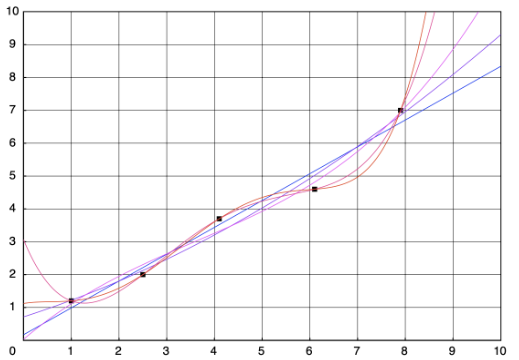
\includegraphics[width=10cm, scale=1]{images/overfitting}
	\caption{Overfitting}
	\label{overfitting}
\end{figure}


\subsection{Unsupervised Models}
L'apprendimento non supervisionato è una categoria di algoritmi di apprendimento automatico che utilizzano dati non etichettati per "imparare" da essi. In contrasto con l'apprendimento supervisionato, dove ci sono dati etichettati con le risposte corrette, l'apprendimento non supervisionato non ha accesso alle risposte corrette, ma cerca di scoprire relazioni o strutture all'interno dei dati.

Ci sono diverse tipologie di algoritmi di apprendimento non supervisionato, tra cui:
\begin{itemize}
\item Clustering: utilizzato per raggruppare gli esempi in base alle loro similitudini.
\item Riduzione della dimensionalità: utilizzato per ridurre la dimensionalità dei dati.
\item Analisi di componenti principali (PCA): utilizzato per individuare le componenti principali dei dati.
\item Apprendimento non supervisionato basato su reti neurali: utilizzato per apprendere rappresentazioni dei dati.
\item Anomaly detection: utilizzato per identificare dati anomali o fuori dalla norma.
\item Generative models: utilizzato per generare nuovi dati.


\end{itemize}
Nel rilevamento supervisionato delle anomalie, se vogliamo che un modello sia in grado di rilevare le anomalie, bisogna allenare il sistema in modo molto preciso sia nell' identificare sia il comportamento normale che quello anomalo.
Tuttavia, i comportamenti normali possono essere molteplici, così come i
comportamenti in presenza di anomalie e questo porta con se la necessità di fornire una grande quantità di dati etichettati per catturare piu comportamenti possibili. Purtroppo non e' sempre possibile in quanto le anomalie sono eventi rari e se il dataset di addestramento e' relativamente piccolo, anche il numero di anomalie non sara' sufficientemente grande, rendendo difficile la loro classificazione. 
Pertanto, l'apprendimento non supervisionato si adatta perfettamente al problema del rilevamento delle anomalie, poiché non è necessario etichettare grandi insiemi di dati. Inoltre, una parte delle anomalie derivano da nuovi comportamenti del sistema e per definizione, questi comportamenti non possono essere classificati correttamente con i metodi di rilevamento delle anomalie supervisionati senza effettuare prima un re-training.


\section{Model Evaluation}
La valutazione del modello è necessaria per quantificarne le prestazioni. La
scelta delle metriche e delle tecniche di valutazione dipende dal task di apprendimento come la classificazione o la regressione. 
In questa sezione ci si concentrerà sulle tecniche e sulle metriche più famose utilizzate per valutare la performance di un modello su un determinato compito.

\subsubsection{Tecniche}
\begin{itemize}
	\item \textbf{Random Split} genera in maniera casuale i tre insiemi di train, test e validazione. Il vantaggio di questo metodo è che c'è una buona probabilità che la popolazione originale sia ben rappresentata in tutti e tre gli insiemi, impedendo quindi un campionamento distorto dei dati.
	\item \textbf{Time Based Split} viene applicato sulle serie temporali in cui non e' possibile effettuare una suddivisione casuale dei dati in quanto si andrebbe a perdere informazioni come trend o seasonality. 
	      In questi casi, si utilizza una suddivisione temporale in cui, ad esempio, l'insieme di train può contenere i dati piu' vecchi, mentre quelli piu' recenti sono assegnati all'insieme di test. Per evitare l'overfitting introdotto da questo metodo, una variante a finestre di scorrimento e' preferibile: il modello viene allenato iterativamente piu' volte su una finestra temporale e valutato sulla parte restante dei dati, per poi allargare la finestra di training ad ogni iterazione (riducendo cosi quella di valutazione).
	\item \textbf{K-Fold Cross Validation} genera in modo casuale $k$ gruppi di dati ed iterativamente vengono usati $k-1$ gruppi per il training ed un gruppo per la valutazione.
	\item \textbf{Stratified K-Fold} e' simile al Cross Validation ma con la differenza che questo metodo tiene in considerazione la distribuzione delle classi dei dati, generando quindi gruppi con rateo simile al dataset originale.
\end{itemize}


\subsubsection{Metriche}
Alla base di tutte le metriche di valutazione vi e' la tabella di contingenza. Questa tabella permette di valutare le performance di un modello andando a relazionare, in piu modi, le predizioni di un modello con i dati di ground-truth.
La tabella \ref{contigency-table} mostra la struttura della tabella di contingenza.  La prima colonna contiene il numero delle predizioni positive fatte da un modello divise se queste sono effettivamente positive o negative. La seconda colonna funziona allo stesso modo ma per le predizione negative dello stesso modello. La terza colonna invece rappresenta la somma dei punti che sono realmente positivi e realmente negativi.
Riassumendo:
\begin{itemize}
\item True Positive: punti realmente positivi che sono predetti come tali
\item False Positive: punti realmente positivi ma predetti come negativi
\item False Negative: punti realmente negativi ma predetti come positivi
\item True Negative: punti realmente negativi che sono predetti come tali
\item Pos: Somma totale dei punti realmente positivi
\item Neg: Somma totale dei punti realmente negativi
\end{itemize}

\begin{table}[]
\centering
	\caption{\label{contigency-table}Tabella di contingenza}

\begin{tabular}{|l|l|l|l|}
\hline
                 & \textbf{Predizioni +} & \textbf{Predizioni -} & \textbf{Totale} \\ \hline
\textbf{Reale +} & TP                    & FP                    & Positivi        \\ \hline
\textbf{Reale -} & FP                    & TN                    & Negativi        \\ \hline
\end{tabular}
\end{table}

A questo punto e' possibile introdurre tutte le misure di performance:
\begin{itemize}
\item Accuracy
\item Error Rate
\item Recall
\item Specificity
\item Precision
\end{itemize}


\section{Thresholding}
iqr, o gammaY del tipo

\section{Machine Learning Models}
\subsection{Linear Models}
\subsection{Distance Based Models}
\subsection{Probabilistic Models}
\subsection{Ensemble Models}

\section{Neural Network Models}
\subsection{Auto Encoders}
\subsection{LSTM}
\subsection{Adversarial Networks}
\subsection{Graph Based}